\chapter{Cosmic rays, the sky model and quality flags}
\label{sec:cosmics}

This chapter comes from a search for the worst reductions of the final pipeline (improved v3). The two worst kinds of
frame were not caused by the steps of the earlier chapters but by two parts of \banzai{} we had not examined: the
cosmic-ray detector (LA Cosmic) and the sky model under the object. In both, the extracted spectrum scatters far more
than its errors. The cosmic-ray detector also clips the peaks of bright emission lines; in one NGC\,4151 frame this
made H$\alpha$ 2.6 times too bright. A cosmic-ray detector can always be tuned to look good on the cases it was tuned
on, so most of the chapter is about testing the changes on data they were not tuned on. The changes are in the code
(branch \texttt{rm-improvements} of \banzai{}), but \textbf{the products of this report have not been re-reduced with
them}; Table~\ref{tab:cr_status} gives the status of each change.

\paragraph{Summary of the chapter.} For each problem: what went wrong, what we changed, how we tested it, and the result.
\begin{itemize}
\item \textit{Bright star cores and emission-line peaks taken for cosmic rays}
(Sections~\ref{sec:cr_method}--\ref{sec:cr_lines}). LA Cosmic in \banzai{}~1.1.0 flags the cores of bright stars and
the peaks of narrow emission lines, and it misses real cosmic rays that land on these bright regions.
\textit{Change} (Section~\ref{sec:cr_model}): before LA Cosmic searches the frame, we subtract a smooth model of the
object (a 7-pixel running median along each detector row), so that only features sharper than the object are left.
\textit{Tests} (Section~\ref{sec:cr_verify}): artificial cosmic rays added to real frames, and a comparison of the two
exposures of each visit for 106 frames. \textit{Result}: in the brightest standard star the flagged share of the core
falls from 46 to 0.1 per cent; on the worst H$\alpha$ line the flagged pixels fall from 179 to 15 and its flux from
2.64 to 1.02 times that of the other exposure; of the artificial cosmic rays above 10$\sigma$ on line peaks and star
cores, 97 instead of 66 per cent are found. The cost is a few more small false detections per frame on the trace of
bright objects (median 1 to 5 per frame at OGG), which do not change the extracted fluxes beyond the noise.
\item \textit{Line peaks that the object model still flags} (Section~\ref{sec:cr_pair}). \textit{Change}: a new
pipeline stage, the \textit{same-visit check}, compares each exposure after LA Cosmic with the other exposure of its
visit and removes flags on features that are present in both. \textit{Tests}: artificial cosmic rays in 8 frames, and
the whole sample of 106 frames. \textit{Result}: it finds the same artificial cosmic rays as the object model alone and
flags 22 (OGG) and 10 (COJ) per cent fewer pixels. It removes the 15 pixels still flagged on the worst H$\alpha$, and
it brings the flagged pixels on the narrow lines of NGC\,4151 to 215, against 236 with \banzai{}~1.1.0 and 398 with
the object model alone.
\item \textit{The sky model beside a wide object} (Section~\ref{sec:cr_sky}). When a wide object leaves little sky in
the slit, the sky model follows the noise and the spectrum scatters 3--4 times its errors. \textit{Change}: a sky line
must also stand out from the scatter of the first-pass sky by 5 robust standard deviations. \textit{Result}: in the affected frames the
scatter falls from 3.0--3.3 to 1.1--1.2 times the errors; in normal frames the flux changes by less than 0.2 per cent.
\item \textit{A guard in the extraction} (Section~\ref{sec:cr_guard}). A wavelength bin that has lost more than half
of its profile weight to cosmic-ray flags is now masked instead of being scaled up from the rest.
\item \textit{Quality keywords} (Section~\ref{sec:qc}). Every product now carries per-frame quality measures and flags
in its header. They were added to all 317 science and standard products of improved v3, and they find the problem
frames that we found by hand in this report.
\end{itemize}

\section{How \banzai{} finds cosmic rays}
\label{sec:cr_method}
\banzai{}~1.1.0 runs LA Cosmic \citep{vanDokkum2001}, as implemented in the Python package \texttt{astroscrappy}, on
each science and standard frame. The names in typewriter font below are the parameters of LA Cosmic. Step by step:
\begin{enumerate}
\item \textit{Sky.} A first sky model $B(x,y)$ is fitted outside a mask around the object trace: a spline in wavelength
times a low-order polynomial along the slit.
\item \textit{Inputs.} LA Cosmic receives the frame $D$ in electrons, its variance from the pipeline's error map, and
$B$ as the background to subtract. It also receives a mask of pixels it must not search: bad pixels, pixels outside the
orders, and a band 2 pixels wide along the edges of each order, because those edges are sharp.
\item \textit{Sharpness.} LA Cosmic subtracts the background, takes the Laplacian of the frame sampled at twice the
resolution, and divides it by the noise: $S=\nabla^2(D-B)/2\sigma$, where $\sigma$ is the noise of the pixel. It then
subtracts the 5-pixel median of $S$ from $S$, to remove its smooth part. A cosmic ray deposits its charge in one or a
few pixels and is far sharper than anything the optics produce, so its $S$ is large.
\item \textit{Candidates.} Pixels with $S>5$ (\texttt{sigclip}) are candidates.
\item \textit{Fine-structure test.} A star or a line is also sharp, but it is as wide as the seeing. LA Cosmic
therefore builds a fine-structure image $F$: the 3-pixel median of the frame minus the 7-pixel median of that. It keeps
a candidate only if its Laplacian is more than 5 times $F$ (\texttt{objlim}).
\item \textit{Growth.} The neighbours of a detected pixel are added to it if their $S$ exceeds
$\texttt{sigfrac}\times\texttt{sigclip}$. \banzai{} uses $\texttt{sigfrac}=0.03$, i.e.\ a threshold of 0.15$\sigma$,
ten times below the LA Cosmic default (0.3). As a result a detection grows over the whole of any bright region it
touches. The detected pixels are replaced by the mean of their unmasked neighbours, and steps 3--6 are repeated four
times.
\item \textit{Fill.} Holes inside a detection are filled in, and its pixels are marked with bit 8 of the mask.
\item \textit{Use.} The sky is fitted again without the flagged pixels, and the extraction leaves them out. In each
wavelength bin the flux is $f=\sum a(d-b)/\sum aP$ over the remaining pixels, where $d$ is the value of a pixel, $b$
the sky model there, $P$ the spatial profile model of the object and $a$ the weight of the pixel in the extraction.
A flagged pixel therefore loses no flux \textit{if the profile model $P$ is right}.
\end{enumerate}

\textit{Which versions do this.} \banzai{}~1.0.1, which made the archive products, has no cosmic-ray detection at all.
The detector of improved v3 is that of \banzai{}~1.1.0 unchanged: the code, its parameters, its place in the order of
pipeline stages and the sky fit before it are identical to the 1.1.0 release. Only its input differs, in two ways.
First, 1.1.0 divides the 2-d frame by the lamp-flat fringe pattern before the detector runs, and improved v3 does not
(Chapter~\ref{sec:fringe}). Second, in improved v3 the object trace that sets the sky mask comes from the physical
trace model (Chapter~\ref{sec:traces}). Neither changes the flags. We checked this on the 46 Fairall~9 frames of the
test of Section~\ref{sec:cr_verify}: \banzai{}~1.1.0 as released (without the object wavelength zero point) and
improved v3 have the same number of real and false detections on the object (136 and 134 real, 1414 and 1420 false),
in the same frames. The problems of this chapter are therefore those of \banzai{}~1.1.0. There is no reduction of OGG
with 1.1.0 as released; since the code is the same, we expect the same star cores and H$\alpha$ to be flagged there.

\section{The core of a bright star taken for cosmic rays}
\label{sec:cr_stars}
The brightest standard star is BD$+28^\circ4211$ at OGG, with peaks of 30\,000--45\,000\,e$^-$ per pixel through the
2\,arcsec slit. In good seeing LA Cosmic flags the core of the star. We measured the share of the trace core (the
pixels within one FWHM of the trace) that is flagged. It is more than 1 per cent in 10 of the 68 spectra of this star
and more than 5 per cent in 6 of them. On 2025 August 19 (seeing 1.3\,arcsec) it is 46 per cent of the core in the blue
order (Fig.~\ref{fig:cr_smoothing}, top). The extraction then works from the wings of the profile, where the profile
model is least right, and the spectrum scatters 2.9 times its errors from bin to bin. No other standard and no AGN frame
is affected: Feige\,110 and the other standards are fainter, and an AGN through a 6\,arcsec slit has a broader profile.
That is why the problem appeared only among the OGG standards.

\section{Emission lines taken for cosmic rays}
\label{sec:cr_lines}
A bright narrow emission line is sharp along the dispersion. In all 160 AGN spectra of improved v3 we looked for flags
on the trace core within $\pm12$\,\AA{} of [O\,{\sc iii}]\,$\lambda\lambda$4959, 5007, H$\beta$ and
H$\alpha$+[N\,{\sc ii}]:
\begin{itemize}
\item \textit{[O\,{\sc iii}]\,5007} is never flagged, in either object.
\item \textit{[O\,{\sc iii}]\,4959.} In one Fairall~9 frame (2026 August 28) five pixels of the core of the line are
flagged. They are false positives, because they agree with the other exposure of the visit within the noise; they have no
measurable effect on the flux.
\item \textit{[O\,{\sc iii}]\,4959 in 12 NGC\,4151 frames.} These flags are a warm detector pixel of the OGG camera at
$(x,y)=(1465,409)$, with 24\,500\,e$^-$ against 500--1000 in its neighbours. It is not in the bad-pixel mask, and it
falls on the wing of the line because NGC\,4151 is always placed at the same position in the slit. Masking it is right.
\item \textit{H$\alpha$ of NGC\,4151} is flagged in 7 of 60 frames, by up to 179 pixels covering the peak of the line
(Fig.~\ref{fig:cr_halpha}). The two exposures of a visit normally agree on the H$\alpha$+[N\,{\sc ii}] flux to 2.5 per
cent. Two exposures with clipped lines had 2.64 and 1.18 times the flux of the other exposure of their visit. In the
other five the flags changed the flux by no more than the noise (one pair differs by 6 per cent with or without flags).
\end{itemize}
The flux is biased upwards, and the bias can be large, because of how the extraction treats flagged pixels
(Section~\ref{sec:cr_method}, step 8). With the core of the line removed, what is left in the bin is the wings of an
emission region that is resolved along the slit (the narrow-line region of NGC\,4151 is extended). Their flux is divided
by the small profile weight of those wings, as if they held the same fraction of the light as in the continuum.
\textit{This can happen in any bright object with strong narrow lines in good seeing}---Seyfert galaxies, H\,{\sc ii}
galaxies, planetary nebulae. It is not visible in the extracted spectrum unless one compares exposures: the spectrum
simply shows an H$\alpha$ that is too strong.

\begin{figure}[!htbp]
\centering
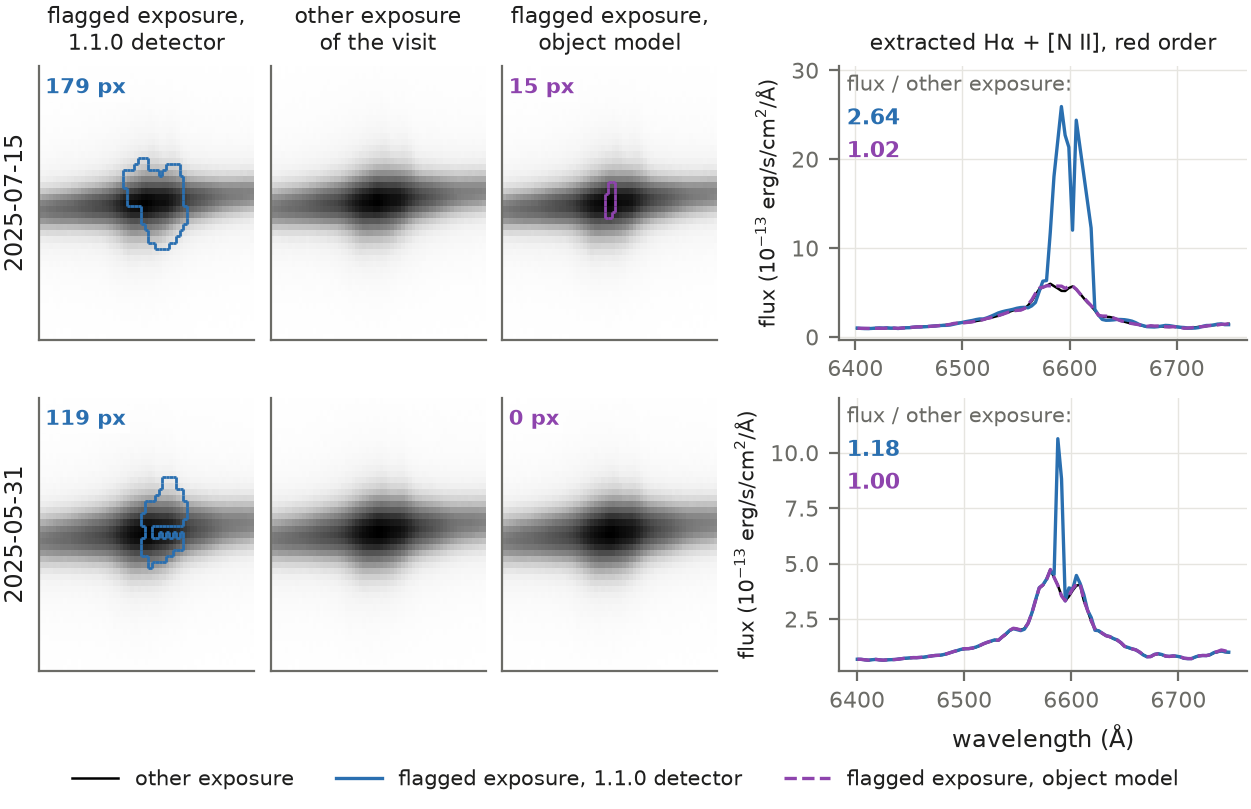
\includegraphics[width=\textwidth]{figures/fig_cr_halpha.png}
\caption{H$\alpha$ of NGC\,4151 flagged as cosmic rays (OGG, 6\,arcsec slit). Left: the 2-d frame around H$\alpha$
(counts, same arcsinh grey scale in a row) of the flagged exposure with the flags of the 1.1.0 detector of improved v3
(blue), the other exposure of the same visit, and the flagged exposure with the object model (purple). Right: the
extracted H$\alpha$, with the H$\alpha$+[N\,{\sc ii}] flux of the flagged exposure divided by that of the other
exposure. Top: 2025 July 15, 179 pixels flagged and the flux 2.64 times too high; with the object model 15 pixels are
flagged, the four bins where they remove most of the profile are masked by the extraction guard
(Section~\ref{sec:cr_guard}) and the ratio is 1.02. Bottom: 2025 May 31, 119 pixels and 1.18; with the object model
none and 1.00.}
\label{fig:cr_halpha}
\end{figure}

\section{A related problem: the sky model beside a wide object}
\label{sec:cr_sky}
\textit{The problem.} The worst Fairall~9 spectra (six frames on 2026 September 3, 6 and 16) scatter 3--4 times their
errors from bin to bin, although their 2-d frames have the noise their error maps predict. The excess is already in the
extraction before any correction, in both the optimal and the unweighted sums, and it is absent from a plain box
sum of the same pixels. It therefore comes from the sky model.

\textit{The cause.} The sky model is a spline in wavelength, with knots one pixel apart on sky lines and three pixels
apart elsewhere. Sky lines are found as the pixels of a first-pass sky model that are more than 15 per cent above its
running median. In these frames the Moon was up (58--80 per cent illuminated) and the seeing was 2.6--4.5\,arcsec, so
Fairall~9 fills much of the slit. The mask that keeps the object out of the sky fit is then narrowed to less than
6 times the width ($\sigma$) of the spatial profile on each side (header keyword \texttt{L1BKMW}\,$<6$), and few sky
pixels are left. The first-pass sky is noisy, its noise passes the 15 per cent test, and nearly every column gets a
knot (1464 instead of $\approx500$). The sky under the object then follows the noise of a few pixels at the edges of
the slit, multiplied by the number of pixels in the extraction window. Two measurements show this. The bin-to-bin
second differences of the extracted flux and of the sky are anticorrelated, with coefficients of $-0.95$ to $-0.97$.
And the sky model scatters by 3.5--3.8 times the flux errors, against 0.1 in normal frames. The same noisy sky also
makes LA Cosmic flag the object: the two frames of 2026 September 3 each have $\approx$240 flagged groups on the object
that are not in the other exposure (Section~\ref{sec:cr_verify}).

\textit{The change.} A sky line must now also stand out from the scatter of the first-pass sky by 5 robust standard
deviations. \textit{Result}: on the affected frames the scatter falls from 3.0--3.3 to 1.1--1.2 times the errors and
the number of knots to $\approx500$. On normal frames the flux changes by less than 0.2 per cent, and the fringe
residual is unchanged or slightly lower.

\section{The change to the detector: a model of the object}
\label{sec:cr_model}
LA Cosmic subtracts the background it is given before it measures sharpness (step 3 above). The documentation of
\texttt{astroscrappy} says that, for spectra, this background should remove the sky lines \textit{and the
cross-section of the object}. \banzai{} gives it the sky only. The object itself is therefore searched for cosmic
rays, and only the fine-structure test (step 5) stands between a bright core and a flag. Our change adds one step
between steps 1 and 2:
\begin{enumerate}
\item[1a.] \textit{Object model.} Take the frame minus the first sky model, $R=D-B$, inside the orders. (Pixels outside
an order take the nearest in-order value of their row, so that the filter does not mix zeros into the ends of an
order.) Along each detector row, replace every pixel by the median of the 7 pixels centred on it:
$M(x,y)=\mathrm{median}\{R(x-3..x+3,y)\}$, set to zero where negative. Give LA Cosmic $B+M$ as the background instead
of $B$.
\end{enumerate}
Everything else (parameters, noise, growth of detections, use in the extraction) is unchanged. LA Cosmic now searches
$D-B-M$. A 7-pixel median along the row treats the three kinds of sharp feature differently:
\begin{itemize}
\item \textit{A cosmic ray} covers 1--5 pixels. The 7-pixel median ignores it, so it stays in $D-B-M$ at full strength
and is found, also on the trace (Fig.~\ref{fig:cr_method}, bottom row). On bright cores and line peaks it is found
more often than before, because the object no longer hides it (Section~\ref{sec:cr_inject}).
\item \textit{A star.} The traces are tilted on the detector, so along one row the core of a star is spread over tens
of columns (about 40 for BD$+28^\circ4211$). This is a smooth hump that the median follows, and $D-B-M$ is noise
(Fig.~\ref{fig:cr_method}, top row: 950 pixels flagged before, 6 after, all on the sky).
\item \textit{A narrow emission line} is narrow along the row too. The median cuts its peak, and part of the peak is
left in $D-B-M$ (Fig.~\ref{fig:cr_method}, middle row). For [O\,{\sc iii}]\,5007 in NGC\,4151 this is 22 per cent of
the peak (Fig.~\ref{fig:cr_smoothing}). That remainder is as wide as the object along the slit, so the fine-structure
test rejects most of it, but not all: 15 pixels of the H$\alpha$ peak of 2025 July 15 are still flagged (180 before).
They are false positives, since the other exposure of the visit has the same line, and the same-visit check of
Section~\ref{sec:cr_pair} removes all 15. This is the weak point of the object model alone, and the reason for that
check and for the extraction guard (Section~\ref{sec:cr_guard}).
\end{itemize}
Figure~\ref{fig:cr_method} shows the steps on identical inputs: the same pixels, sky, errors and parameters, with LA
Cosmic given either $B$ (as in 1.1.0) or $B+M$. The flag counts in the figure reproduce those of the reductions: 180
H$\alpha$ pixels against 179 in improved v3, and 15 against 15 with the new code.

\textit{Alternatives tried.}
(i) Restoring the LA Cosmic default $\texttt{sigfrac}=0.3$ without the object model. The flagged share of the star core
falls only from 40 to 36 per cent, and the H$\alpha$ flags from 180 to 109 pixels: the setting limits the growth of a
detection but does not stop the core being detected. Together with the object model it reduces the flags further
(H$\alpha$: 13 pixels), but it also shrinks the masks of real cosmic rays (from 18 to 9 pixels), possibly leaving their
faint edges unmasked. We kept 0.03 until the injection test settles the question.
(ii) Raising $\texttt{objlim}$ from 5 to 15 changed nothing for the star cores.
(iii) An object model built from the fitted spatial profile (profile $\times$ flux of each bin), which keeps the lines
at full resolution. It flagged up to 80 pixels of [O\,{\sc iii}] in NGC\,4151, whose narrow-line region has a
different spatial profile from the continuum, and raised the line flux by 10--16 per cent. We rejected it.

\begin{figure}[!htbp]
\centering
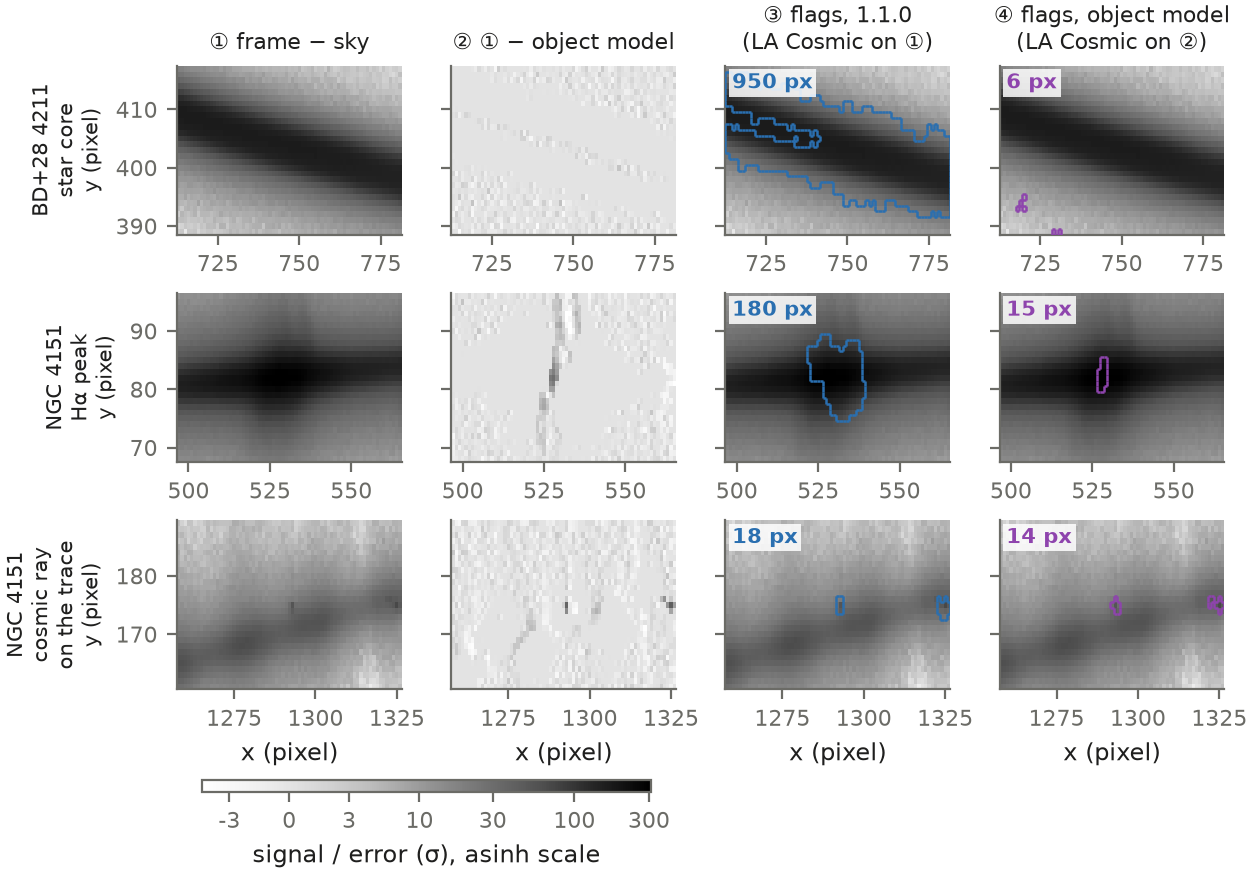
\includegraphics[width=\textwidth]{figures/fig_cr_method.png}
\caption{The change step by step on identical inputs. Columns: \ding{172} the frame minus the sky, which the 1.1.0
detector searches; \ding{173} the same minus the object model (the 7-pixel running median along each detector row),
which LA Cosmic searches with the change; both in units of the error, on one grey scale; \ding{174} the pixels flagged
when LA Cosmic is given only the sky (\banzai{}~1.1.0 and improved v3, blue) and \ding{175} when it is given the sky
and the object model (purple), with the number of flagged pixels in the panel. Rows: the core of BD$+28^\circ4211$ in
1.3\,arcsec seeing (2025 August 19): 950 pixels against 6, all on the sky; the H$\alpha$ peak of NGC\,4151 (2025 July
15): 180 against 15; a real cosmic ray on the trace of NGC\,4151 (2025 July 19), found both ways. The 15 H$\alpha$
pixels still flagged with the object model are false positives, removed by the same-visit check
(Fig.~\ref{fig:cr_pair}).}
\label{fig:cr_method}
\end{figure}

\begin{figure}[!htbp]
\centering
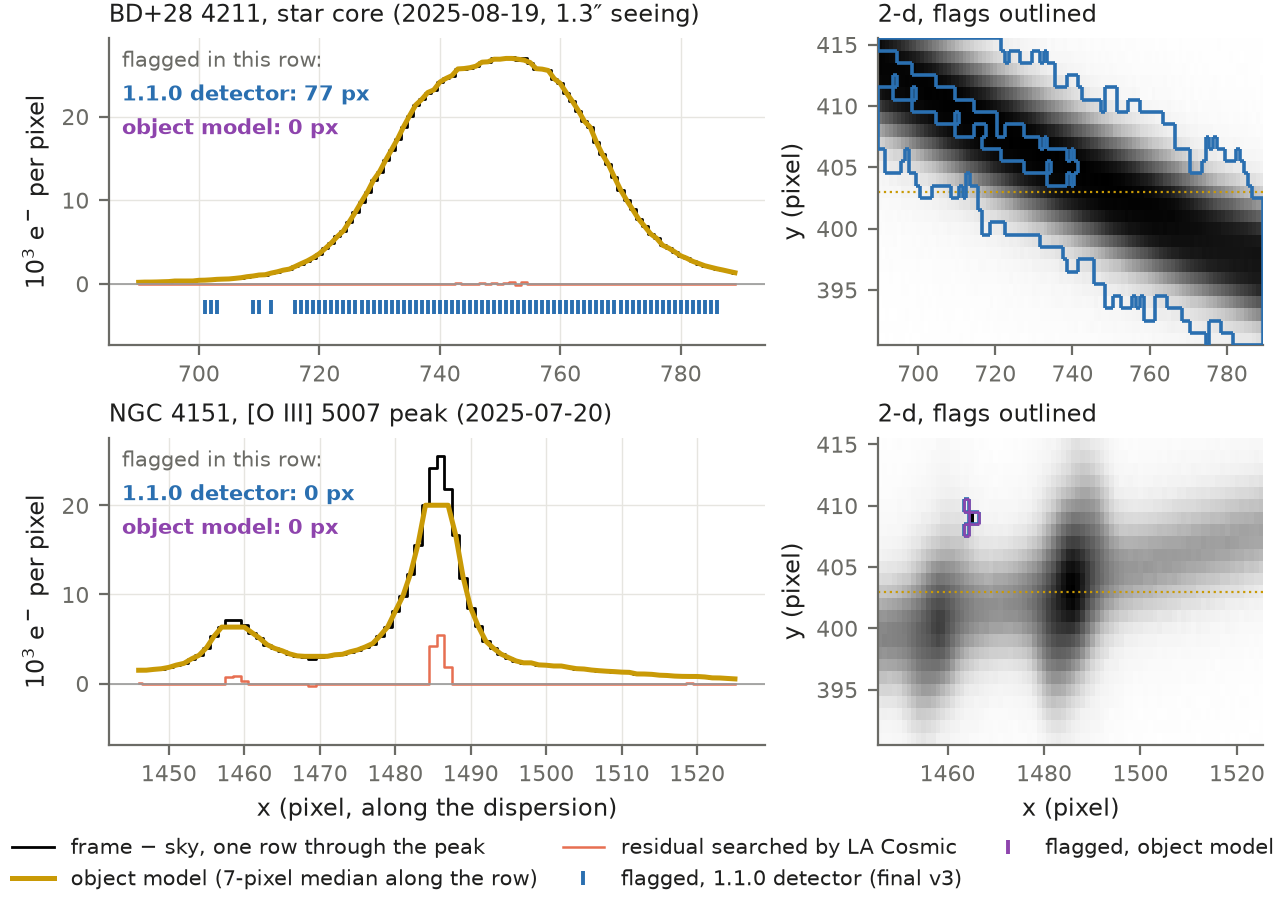
\includegraphics[width=\textwidth]{figures/fig_cr_smoothing.png}
\caption{What the object model does. Left: one detector row through the core of BD$+28^\circ4211$ (top, blue order,
2025 August 19) and through the peak of [O\,{\sc iii}]\,5007 of NGC\,4151 (bottom, 2025 July 20): frame minus sky
(black), the object model, a 7-pixel median along the row (gold), the residual that LA Cosmic searches (orange), and
the pixels flagged in that row by the 1.1.0 detector of improved v3 (blue ticks) and with the object model (purple
ticks); the counts are written in the panel. Right: the 2-d frame (arcsinh grey scale) with the same flags outlined
and the row of the left panel dotted. The flag near $x=1465$ is the warm pixel of the OGG camera, flagged by both.}
\label{fig:cr_smoothing}
\end{figure}

\section{A safety net in the extraction}
\label{sec:cr_guard}
Whatever the detector does, the extraction should not turn a few flagged pixels into a flux error of a factor 2.6. For
each wavelength bin we therefore measure the share of the profile weight in the extraction window ($\sum aP$ of
step 8, Section~\ref{sec:cr_method}) that belongs to pixels flagged as cosmic rays. A single real cosmic ray on the
trace removes at most 0.48 of it (0.15--0.42 for the artificial cosmic rays of Section~\ref{sec:cr_inject}, and 0.48 in
the worst standard star). The clipped H$\alpha$ bins lose 0.51--0.75, even with the new detector. Bins where more than
half of the weight is removed are now masked in the extracted spectrum instead of being scaled up from the rest. We
call this the \textit{extraction guard}. It sets bit 4 of the mask of the extracted spectrum (\texttt{EXTRACTED}
extension), stores the share in a new column \texttt{cr\_masked\_weight}, and counts the masked bins in the header
keywords \texttt{L1QCRB1} and \texttt{L1QCRB2} (red and blue order). A masked bin is not recovered, but it is visible.

% Same-visit cosmic-ray check (banzai_floyds/visit_cosmics.py), input from ch11_cosmics.tex
\section{The second exposure of the visit}
\label{sec:cr_pair}
\textit{The problem.} With the object model, LA Cosmic searches the right residual, but it still has to judge a sharp
feature by its shape alone. A narrow line from a resolved narrow-line region can be as sharp as a cosmic ray (the 15
H$\alpha$ pixels of Fig.~\ref{fig:cr_method}). \textit{The idea.} The visits of the reverberation-mapping programme have
two exposures of the same pointing, taken back to back. A cosmic ray lands in only one of them; a line, a star core, a
sky line or a fringe is in both. The other exposure of the visit (the \textit{partner}) is therefore the most direct
test there is. \textit{The change.} We have added this test to the pipeline as a stage that runs right after LA Cosmic
and that we call the \textit{same-visit check} (code: \texttt{SameVisitCosmicRays} in
\texttt{banzai\_floyds/visit\_cosmics.py}). It removes the LA Cosmic flags on features that the partner also shows,
and adds strong, compact hits that LA Cosmic missed. \textit{Tests and result}
(Sections~\ref{sec:cr_pair_inject} and \ref{sec:cr_pair_sample}): it finds the same artificial cosmic rays as the
object model alone, flags 10--22 per cent fewer pixels, and clears the H$\alpha$ peak of
Fig.~\ref{fig:cr_halpha}.

For a frame $a$ with partner $b$, the check does the following.
\begin{enumerate}
\item \textit{Find the partner}: among the raw frames of the same night in the folder of the frame, those of the same
type and the same LCO \textit{molecule} (the group of exposures taken together within one request; header keyword
\texttt{MOLUID}), the nearest in time first. A frame without a partner keeps the LA Cosmic flags of
Section~\ref{sec:cr_model}. This is the case for all the standards, which are single exposures.
\item \textit{Reduce the partner} up to and including LA Cosmic, in the same way as the frame (no database records are
written for it). Each exposure is sky-subtracted with its own sky model.
\item \textit{Shift the partner along the slit} onto the trace of the frame. The shift is the difference of the fitted
trace centres in each column, smoothed over 15 columns. Where the object is bright (S/N of the column above 30), it is
refined by the difference of the flux centroids within 2\,FWHM of the trace, smoothed over 5 columns. This refinement
is needed because the trace centres follow the continuum, while the narrow-line region of NGC\,4151 can sit up to half a
pixel away, and a half-pixel offset turns the peak of a bright line into a positive--negative pattern in the difference
with the partner.
\item \textit{Scale the partner} in each column by the median ratio $a/b$ over the trace core, smoothed over 31
columns. Where the object is faint, the ratio of the exposure times is used.
\item \textit{Shift the partner along the dispersion.} In a wide slit, the position of the object across the slit
shifts its spectrum. The two exposures of a visit differ by 0.1\,pixel (median) at OGG and 0.3\,pixel at COJ, and by up
to 0.6 and 1.2\,pixels; this puts the flanks of a bright narrow line out of step. The offset is measured for each order
from the cross-correlation of the two spectra summed over the trace (a parabola through its peak). Where it exceeds
0.1\,pixel, it is removed by resampling the partner with a cubic spline. The offset is used only where the peak of the
normalised cross-correlation exceeds 0.5, because a spectrum with no features above the noise has no offset to measure
(Section~\ref{sec:cr_pair_sample}). It is recorded in the header keywords \texttt{L1CRDX1} and \texttt{L1CRDX2} (red
and blue order).
\item \textit{Match the partner to the frame.} The seeing changes within a visit. For example, the FWHM of Fairall\,9
went from 11.6 to 14.7\,pixels between the two exposures of 2026 September 6 (and its flux changed by a factor 0.63);
a scale and a shift cannot absorb that. As in image subtraction \citep{Alard1998}, the partner is therefore convolved
with a kernel along the slit, fitted to the frame:
\[
m(y)=\sum_{|k|\le6}c_k\,s\,b(y+k)+c_{\rm sky}+c'_{\rm sky}\,y ,
\]
where $m$ is the matched partner, $y$ the pixel along the slit, $s$ the scale of step 4, $c_k$ the kernel for an offset
of $k$ pixels, and $c_{\rm sky}$ and $c'_{\rm sky}$ a constant and a slope that absorb a difference between the two sky
models. The kernel is fitted on blocks of 15 columns, on both exposures median-filtered over those columns, with
4$\sigma$ clipping. The median filter is needed for two reasons: a fit on the noisy partner itself is biased towards
zero, and the filter keeps cosmic rays out of the fit. The kernel is then applied to the unfiltered partner, after its
flagged and masked pixels have been replaced by the filtered values. Without this replacement the kernel, which has
negative side lobes when it sharpens the profile, would print a negative copy of a cosmic ray of the partner next to
it. A kernel shared by 15 columns cannot reproduce a hit of a pixel or two, so the matching does not remove real cosmic
rays from the comparison.
\item \textit{Compare}: each pixel gets the significance of its excess over the matched partner,
\[
z=\frac{a-m}{\sqrt{\sigma_a^2+\sigma_m^2+(f\,m)^2}},\qquad f=0.01,
\]
where $\sigma_a$ is the error of the frame, $\sigma_m$ the error of the partner propagated through the kernel, and $f$
a tolerance of 1 per cent for imperfect matching. Each pixel also gets its excess relative to the signal under it,
$r=(a-m)/m$ (with $m$ taken as at least 3 times the denominator of $z$).
\item \textit{Decide}, starting from the LA Cosmic flags. A connected group of flagged pixels is called a
\textit{group}.
\begin{itemize}
\item \textit{Confirm or remove.} A group is \textit{confirmed} if its largest $z$ is at least 3. Otherwise the partner
shows the same feature, and the group is \textit{removed}.
\item \textit{Trim.} Of a confirmed group, only the pixels with $z\ge3$ and their neighbours stay flagged. This prevents
a line peak that LA Cosmic merged with a cosmic ray beside it from being clipped with it.
\item \textit{Pixels the partner cannot check.} Such a pixel always stays flagged, and a group made mostly of such pixels
stays flagged in full. The partner cannot check a pixel that is masked in it; a pixel that it also flags, if the pixel
is off the object (this is how a warm pixel looks); a pixel at the edge of an order; or a pixel where the matched
partner differs from the frame over an extended area (the median of $|z|$ over $5\times5$ pixels is above 2). Such
extended differences occur because the residual 2-d fringes of the red order stay at the same place on the detector
while the partner is shifted onto the trace of the frame, and because the match can fail at the end of an order. A
cosmic ray is compact, so an extended difference says nothing about one. This affects 0.04--4 per cent of an order in
the frames we examined (header keyword \texttt{L1CRMISM}).
\item \textit{Pixels flagged in both exposures, on the object.} LA Cosmic flags the same sharp line and trace peaks in
both exposures of a good-seeing visit. If neither exposure could check the other, both would keep these false flags.
Therefore, on the object (within 2\,FWHM of the trace), a pixel that the partner also flagged is still compared with
the partner's own value, with the kernel applied to the partner without the replacement of step 6. If the two agree,
the pixel holds the same feature in both exposures, since a cosmic ray does not hit the same pixel twice, and the flag
is removed. If the partner is brighter by more than 3$\sigma$, the partner was hit there, and the pixel counts as one
the partner cannot check. No new flags are added on such pixels. Off the object this rule does not apply: a warm pixel
is also in both exposures, and on the sky nothing distinguishes it from a real feature. The header keyword
\texttt{L1CRSHAR} counts the pixels the rule is applied to.
\item \textit{New groups}, the cosmic rays LA Cosmic missed, must pass a stricter test than confirmations, because on a
bright line a mismatch of 1 per cent of the partner is already many $\sigma$. A new group starts from a pixel that
meets all of the following: $z>8$; $r>0.5$, i.e.\ at least 50 per cent above the signal under it; significantly
positive itself, $a>5\sigma_a$ (a cosmic ray adds charge); and at least 6 pixels from the edges of an order along the
slit and from its ends along the dispersion. The group is then extended into neighbouring pixels with $z>3$ and
$a>2\sigma_a$. It is accepted only if the result is compact: at most 30 pixels, 3 pixels thick and 15 long.
\end{itemize}
\end{enumerate}
The result is recorded in the header of every product:
\begin{itemize}
\item \texttt{L1CRMETH}: \texttt{pair} if the frame was checked against a partner, \texttt{lacosmic} if not;
\item \texttt{L1CRPART}: the file name of the partner;
\item \texttt{L1CRNLA}: the number of pixels flagged by LA Cosmic;
\item \texttt{L1CRKEEP}, \texttt{L1CRDROP}, \texttt{L1CRUNCH} and \texttt{L1CRADD}: the number of groups confirmed,
removed, kept because the partner could not check them, and added;
\item \texttt{L1CRNPX}: the number of pixels flagged at the end;
\item \texttt{L1CRMISM}: the fraction of the orders that the partner cannot judge because of extended differences;
\item \texttt{L1CRSHAR}: the number of pixels on the trace flagged by LA Cosmic in both exposures and judged against
the partner's own values;
\item \texttt{L1CRDX1} and \texttt{L1CRDX2}: the offset of the partner along the dispersion, in pixels, for the red and
blue orders.
\end{itemize}

\textit{The tolerance $f$} was measured, not chosen. We used the trace cores of two pairs: the bright NGC\,4151 visit
of 2025 July 14 at OGG (FWHM 4.6 and 4.9\,pixels) and the Fairall\,9 visit of 2026 September 6 described above. If the
errors are right, the robust scatter of $z$ should be 1 (Table~\ref{tab:cr_pair_tol}). With $f=0$, $z$ scatters by
0.8--1.1 at every signal level up to $3\times10^4$\,e$^-$ per pixel (up to 1.4 at COJ, where the object is faint), and
by 1.1--1.2 above that. With $f=0.01$ the scatter of the brightest pixels falls to 0.7, and 0.1 per cent of the core
pixels have $|z|>3.8$--4.1. Without the kernel, $z$ scatters by up to 2.9 (OGG) and 3.4 (COJ) even with a 2 per cent
tolerance, mostly because of the change of seeing. Our first version used tolerances of 5 per cent in flux and
0.25\,pixel in position, chosen by hand to absorb that change. With them $z$ scattered by only about 0.3 on bright
pixels, which hid the weaker hits on bright lines from the comparison.

\begin{table}[!htbp]
\centering\small
\caption{Robust scatter of $z$ on the trace core of two clean pairs, by the signal of the matched partner (e$^-$ per
pixel), with the tolerance adopted ($f=0.01$; partner shifted along the dispersion and matched by the kernel). It
should be 1. The numbers before the arrow are for a scale and a shift along the slit only, with $f=0.02$.}
\label{tab:cr_pair_tol}
\begin{tabular}{lccccc}
\toprule
Pair (frame vs partner) & $<10^3$ & $10^3$--$3\times10^3$ & $3\times10^3$--$10^4$ & $10^4$--$3\times10^4$ & $>3\times10^4$\\
 & \multicolumn{5}{c}{signal of the matched partner (e$^-$ per pixel)} \\
\midrule
NGC\,4151 OGG, 0002 vs 0001 & 1.29$\to$0.83 & 2.17$\to$0.90 & 2.92$\to$0.91 & 1.63$\to$0.83 & 2.60$\to$0.73\\
NGC\,4151 OGG, 0001 vs 0002 & 1.15$\to$0.85 & 1.31$\to$0.84 & 1.53$\to$0.85 & 1.02$\to$0.81 & 1.22$\to$0.66\\
Fairall\,9 COJ, 0014 vs 0013 & 1.93$\to$1.00 & 2.49$\to$0.76 & -- & -- & --\\
Fairall\,9 COJ, 0013 vs 0014 & 1.86$\to$1.02 & 3.44$\to$0.93 & --$\to$1.31 & -- & --\\
\bottomrule
\end{tabular}
\end{table}

\textit{What the tests found while building the check.} Each step above was added because a test failed without it,
and each failure now has its own unit test (16 tests in \texttt{tests/test\_visit\_cosmics.py}).
\begin{enumerate}
\item[(i)] The first version (scale and shift only, with the hand-set tolerances of 5 per cent and 0.25\,pixel) lost
weak hits on bright line peaks in the injection test. The tolerances were hiding the change of seeing; matching the
seeing (step 6) fixed that.
\item[(ii)] The kernel printed negative copies of the partner's cosmic rays: 12 false groups in one Fairall\,9 frame.
Replacing those pixels before the convolution fixed it.
\item[(iii)] A warm pixel flagged in both exposures was unflagged in one of them, because its neighbours, which the
partner could check, agreed. Such pixels now always stay flagged.
\item[(iv)] The first run on the whole sample \textit{added} flags on the narrow lines of NGC\,4151 (840 pixels in 41
of 60 frames), more than the object model alone. Three effects produced excesses that the first, loose rule for new
groups ($z>6$ and 10 per cent above the signal) took for cosmic rays: the offsets along the dispersion; an empty frame
compared with a partner that the kernel had made negative at the order edges; and the unmatched 2-d fringes. The
answers are the shift along the dispersion (step 5), the stricter rule for new groups, and the exclusion of extended
differences. On the four worst frames, the flags on the lines went from 9--23 pixels with the object model to 0--6
kept or added pixels, except in one frame (2025 June 10), where 21 LA Cosmic pixels on the lines are kept and 5 added.
\item[(v)] The run of that version on the whole sample still left 215 flagged pixels on the lines of NGC\,4151, a
hundred times the rate on the continuum next to them, and often on the same line in both exposures of a visit. The
partner had flagged the same peak, so neither exposure could check the other. The rule for pixels flagged in both
exposures on the object is the answer (Section~\ref{sec:cr_pair_sample}). Applied everywhere, the rule also unflagged
warm pixels on the sky, which is why it stops at 2\,FWHM from the trace.
\end{enumerate}
Two refinements that looked right on simulations were measured on the real pairs and dropped: a kernel along the
dispersion, which made the tails of the distribution of $z$ worse, and a wider median filter for the kernel along the
slit, which followed the change of the profile along the order too coarsely.

\begin{figure}[!htbp]
\centering
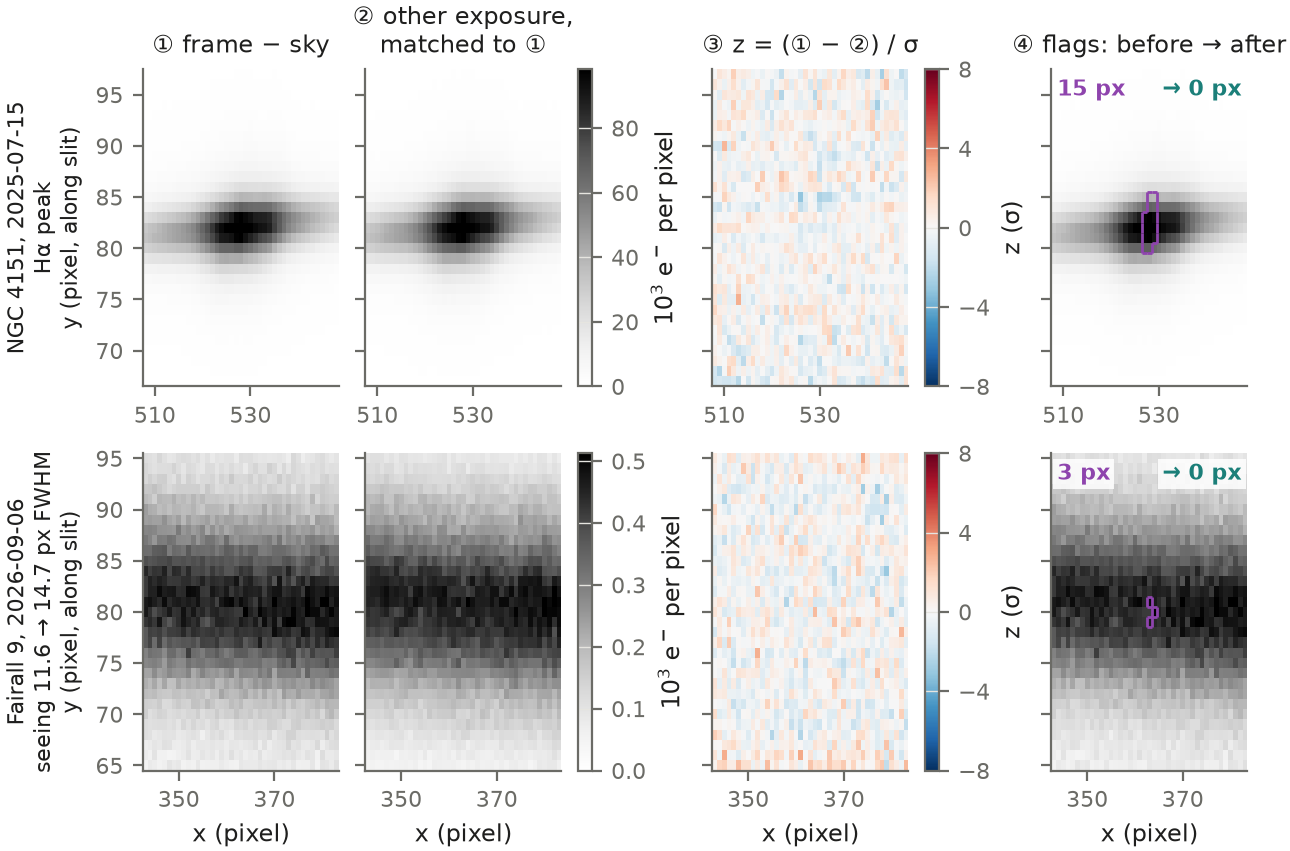
\includegraphics[width=\textwidth]{figures/fig_cr_pair.png}
\caption{The same-visit check on real pairs, both exposures reduced exactly as the stage sees them. Columns:
\ding{172} the frame minus its sky; \ding{173} the partner minus its sky, shifted onto the trace of the frame, scaled
per column, shifted along the dispersion and matched to the frame by the kernel along the slit (same grey scale as
\ding{172}); \ding{174} $z=($\ding{172}$-$\ding{173}$)/\sigma$, which is noise only where the two exposures show the
same thing; \ding{175} the flags of LA Cosmic with the object model (purple, before the check) and those left after the
check (teal; none here), with the number of flagged pixels in the panel. Rows: the H$\alpha$ peak of NGC\,4151 on 2025
July 15 (Figs.~\ref{fig:cr_halpha}, \ref{fig:cr_method}), 15 pixels removed; an LA Cosmic group on the trace of
Fairall\,9 that the partner shows to be real structure, in the visit where the FWHM changed from 11.6 to
14.7\,pixels, 3 pixels removed.}
\label{fig:cr_pair}
\end{figure}

% Results of the same-visit check (input from cr_pair.tex)
\subsection{Injection test with a partner}
\label{sec:cr_pair_inject}
We repeated the injection test of Section~\ref{sec:cr_inject} on eight frames that have a partner: four of NGC\,4151
at OGG and four of Fairall\,9 at COJ. In each frame we placed two random sets of 20 artificial cosmic rays in each of three
places: on the sky, on the trace, and on the line peaks or core. As real cosmic rays
are, they were injected into one exposure of the visit only. Each frame was then reduced three ways: with the 1.1.0
detector, with LA Cosmic and the object model, and with the object model followed by the same-visit check
(Table~\ref{tab:cr_pair_inject}).

\begin{table}[!htbp]
\centering\small
\caption{Injection test on frames with a partner: fraction of injected hits found (any pixel flagged), all hits and
those above 10 times the noise of their pixel, and the cosmic-ray pixels flagged in the same four frames without
injection. 160 hits per category and site (153 on the OGG peaks).}
\label{tab:cr_pair_inject}
\begin{tabular}{llccccc}
\toprule
Site & Detector & Sky & Trace & Line peak & Line peak & Pixels flagged \\
 & & & & or core & or core, $>10\sigma$ & without injection \\
 & & \multicolumn{4}{c}{(fraction of the hits detected)} & (pixels, 4 frames) \\
\midrule
OGG & 1.1.0 / improved v3 & 0.89 & 0.59 & 0.14 & 0.27 & 1037\\
    & object model & 0.89 & 0.76 & 0.50 & 0.89 & 1020\\
    & object model + same visit & 0.89 & 0.76 & 0.50 & 0.89 & 799\\
\midrule
COJ & 1.1.0 / improved v3 & 0.90 & 0.94 & 0.68 & 0.94 & 1775\\
    & object model & 0.90 & 0.94 & 0.79 & 1.00 & 1816\\
    & object model + same visit & 0.90 & 0.94 & 0.78 & 1.00 & 1634\\
\bottomrule
\end{tabular}
\end{table}

\textit{Result.} With the strict rule for new groups, the check finds the same artificial cosmic rays as the object
model alone. Of the 953 hits, none is found only with the check, and 2 are found only without it; both are faint hits on
Fairall\,9 line peaks (3.7--5$\sigma$, 7--12 per cent of the line). On the OGG line peaks, 8 hits above 10$\sigma$ are
missed by both; they carry 4--38 per cent of the line under them. An earlier version of the check, with the loose rule
for new groups, found 14 more hits on the sky and 6 more on the line peaks. But the same rule added hundreds of false
pixels on the narrow lines of the real sample (Section~\ref{sec:cr_pair}, item (iv)), and we chose clean lines.

What the check does is remove flags. In the frames without artificial cosmic rays it flags 22 per cent fewer pixels at
OGG and 10 per cent fewer at COJ. Per frame, it removes 9--19 LA Cosmic groups that the partner shows to be real
structure and adds 0--1; 35--51 groups per frame stay flagged because the partner cannot check them.

These runs were made before the rule for pixels flagged in both exposures on the object was added. That rule acts only
where the partner flagged the same pixel, and an artificial cosmic ray is in one exposure only, so the rule does not
change which of them are found.

% Same-visit check on the whole sample (input from cr_pair_results.tex)
\subsection{The whole sample}
\label{sec:cr_pair_sample}
We reduced all 106 exposures of the sample again with the check (60 of NGC\,4151 at OGG, 46 of Fairall\,9 at COJ).
Every one found its partner (\texttt{L1CRMETH} = \texttt{pair}). These products were made with the version of the
check \textit{before} the rule for pixels flagged in both exposures on the object (Section~\ref{sec:cr_pair}, step 8).
That rule was added after this run and measured on the seven frames with the most flags left on the lines; the sample
was not reduced again. Below, we call the version run on the sample the \textit{sample version}, and each number says
which version it comes from.

\paragraph{Flags on the narrow lines.} Table~\ref{tab:cr_pair_lines} counts the flagged pixels within 12\,\AA\ of
[O\,\textsc{iii}]\,$\lambda\lambda$4959,\,5007, H$\beta$ and H$\alpha$+[N\,\textsc{ii}] and within 8\,pixels of the
trace. On the NGC\,4151 lines, the first version of the check doubled the flags of the object model. The sample
version brings them to 215, fewer than with the object model alone (398) and with 1.1.0 (236), and it clears most of
the H$\alpha$ flags of 1.1.0. Fairall\,9 has few flags on its lines with any detector.

Most of these 215 pixels are still not cosmic rays. They are 0.32 per cent of the pixels in the line windows, against
0.003 per cent in five continuum windows on the same traces. Often both exposures of a visit are flagged at the same
line, which a cosmic ray cannot do. We found two causes in the worst frames. First, in good-seeing visits LA Cosmic
flags the same line and trace peaks in both exposures, so neither can check the other (item (v) of
Section~\ref{sec:cr_pair}). Second, on tilted lines a residual offset between the exposures leaves a
positive--negative pattern, whose positive half passes as a confirmed cosmic ray. The rule for pixels flagged in both
exposures removes the first cause (Table~\ref{tab:cr_pair_worst}). We left the second, because a rule for it would be
one more cut tuned on the frames it is meant to fix.

\begin{table}[!htbp]
\centering\small
\caption{Pixels flagged as cosmic rays on the narrow lines of the sample (within 12\,\AA\ of the line and 8\,pixels of
the trace), by order (1 red, 2 blue), for the 1.1.0 detector (improved v3 products), LA Cosmic with the object model, the
first version of the same-visit check, and the version run on the sample (before the rule for pixels flagged in both
exposures). Last rows: total, and frames with any flagged pixel.}
\label{tab:cr_pair_lines}
\begin{tabular}{llcccc}
\toprule
Target & Line, order & 1.1.0 & Object model & Check, first & Check, sample \\
 & & \multicolumn{4}{c}{(pixels)} \\
\midrule
NGC\,4151 & H$\alpha$+[N\,\textsc{ii}], 1 & 211 & 70 & 55 & 20 \\
(60 frames) & H$\beta$, 1 & 1 & 56 & 117 & 28 \\
 & H$\beta$, 2 & 0 & 6 & 0 & 0 \\
 & [O\,\textsc{iii}]\,4959, 1 & 0 & 42 & 71 & 31 \\
 & [O\,\textsc{iii}]\,4959, 2 & 24 & 74 & 139 & 45 \\
 & [O\,\textsc{iii}]\,5007, 1 & 0 & 89 & 170 & 77 \\
 & [O\,\textsc{iii}]\,5007, 2 & 0 & 61 & 288 & 14 \\
 & total & 236 & 398 & 840 & 215 \\
 & frames with any & 18 & 37 & 41 & 28 \\
\midrule
Fairall\,9 & total & 12 & 29 & 21 & 15 \\
(46 frames) & frames with any & 2 & 6 & 4 & 4 \\
\bottomrule
\end{tabular}
\end{table}

\begin{table}[!htbp]
\centering\small
\caption{The rule for pixels flagged in both exposures on the seven NGC\,4151 frames with the most flags on the
lines: pixels on the lines (as in Table~\ref{tab:cr_pair_lines}) flagged by LA Cosmic with the object model, by the
version run on the sample, and with the rule; and the LA Cosmic groups kept because the partner cannot check them
(mostly warm pixels, which the rule must not touch).}
\label{tab:cr_pair_worst}
\begin{tabular}{lccccc}
\toprule
Frame & \multicolumn{3}{c}{Pixels on the lines} & \multicolumn{2}{c}{Groups the partner cannot check} \\
 & LA + object model & sample version & with the rule & sample version & with the rule \\
\midrule
2025-03-27 0021 & 32 & 33 & 20 & 56 & 47 \\
2025-03-27 0020 & 24 & 19 & 13 & 56 & 48 \\
2025-05-31 0020 & 18 & 15 & 12 & 35 & 32 \\
2025-06-10 0006 & 21 & 26 & 22 & 6 & 5 \\
2025-06-10 0007 & 18 & 16 & 16 & 5 & 5 \\
2025-07-05 0004 & 17 & 14 & 14 & 23 & 23 \\
2025-07-14 0002 & 23 & 0 & 0 & 34 & 30 \\
\bottomrule
\end{tabular}
\end{table}

The rule is restricted to the object for a reason. When we applied it everywhere, it took the groups the partner
cannot check from 56 to 0 in the first frame of Table~\ref{tab:cr_pair_worst}. Cutouts showed that the extra groups it
removed off the trace were single warm pixels present in both exposures. On the object, the rule removes only line and
trace peaks, but it will also unflag a warm pixel that happens to lie on the trace. From the density of warm pixels
flagged in both exposures on the sky, we expect 4--7 such groups per frame. Each adds 50--90\,e$^-$ (at most
340\,e$^-$) to a column of the trace, which holds 30\,000--70\,000\,e$^-$ (6000\,e$^-$ in its faintest tenth): typically 0.1--0.3 per
cent of one of the 1700 columns, and at most $\approx6$ per cent (340\,e$^-$ in a column of 6000\,e$^-$). A map of the warm pixels, made from the flags that recur at the same place on the
detector in many frames, would remove them properly; we leave it for later.

\paragraph{The header keywords.} The keywords of the check give, per frame (median, with the range in brackets):
\begin{itemize}
\item \textit{OGG}: LA Cosmic flags 242 (115--715) pixels, of which 188 (96--681) remain after the check (80 per cent,
summed over all frames). 9 groups are confirmed, 12 removed, 34 kept because the partner cannot check them, and 0 (at
most 6) added. The partner cannot judge 0.1 per cent of the orders (at most 6 per cent). The offset along the
dispersion is at most 0.6\,pixel.
\item \textit{COJ}: 321 (175--1755) pixels flagged by LA Cosmic become 278 (129--1519), 90 per cent. 14 groups are
confirmed, 11 removed, 47 kept and 1 (at most 3) added. The partner cannot judge 0.2 per cent of the orders (at most
2.5 per cent).
\end{itemize}

\paragraph{Two faults found on the sample, and fixed.} The sample numbers in this section were measured before these
fixes.
\begin{enumerate}
\item[(i)] \textit{Spurious offsets along the dispersion.} In the blue order of six Fairall\,9 frames, the offset of
the partner along the dispersion came out at 1.4--3.4\,pixels, with the same sign for both exposures of a visit (2026
October 26: $-2.05$ and $-2.05$\,pixels; September 30: $-3.37$ and $-1.52$). A real offset cannot do this: if $b$ is
shifted with respect to $a$, then $a$ is shifted by the opposite amount with respect to $b$. The faint blue spectrum of
Fairall\,9 has no features above the noise. There the normalised cross-correlation peaks at only 0.09--0.26, against
0.92--1.00 in its red order and in both orders of NGC\,4151, and its peak lands wherever the noise puts it: leaving the
flagged cosmic-ray pixels out of the correlation moved one offset from $-2.05$ to $+2.22$\,pixels. An offset is now
used only where the peak exceeds 0.5, which separates the two groups cleanly.
\item[(ii)] \textit{New groups at the end of an order.} In the same frames the check added groups of 1--9 pixels right
at the end of the blue order (1\,pixel from it). There the signal stops sharply, and the matched partner misses the
step by a pixel. The 6-pixel margin in which no new group is added covered the edges of the orders along the slit, but
not their ends along the dispersion. It now covers the ends too.
\end{enumerate}
Measured again on the affected frames, the spurious offsets are gone (the red order keeps its offsets of
0.05--0.24\,pixel), and no group is added at an order end. The flags on the lines of the NGC\,4151 frames of
Table~\ref{tab:cr_pair_worst} are unchanged. Both faults have their own unit test (16 in all).

\paragraph{Fluxes.} What matters in the end is the flux. Table~\ref{tab:cr_pair_flux} gives the robust scatter of the
flux ratio of the two exposures of each visit, for the narrow lines and two continuum windows. This scatter is set by
the slit losses and the seeing, and the choice of detector changes it by 0.5 per cent or less. The one larger change,
for the red-order [O\,\textsc{iii}] of NGC\,4151 with the object model alone (2.5 against 1.7 per cent), is mostly
undone by the check (2.0 per cent). The optimal extraction rebuilds a masked pixel from the profile, so a false flag on
a line peak costs little flux, while a missed cosmic ray costs more. The gain that matters for the light curves is
therefore that of the object model: of the hits above 10$\sigma$ on the OGG line peaks, it finds 89 per cent, where
1.1.0 found 27 per cent (Table~\ref{tab:cr_pair_inject}). The same-visit check is a clean-up on top: 10--22 per cent
fewer flagged pixels (22 at OGG, 10 at COJ), a clean H$\alpha$ peak, and a mask that can be trusted on the lines.

\begin{table}[!htbp]
\centering\small
\caption{Robust scatter of the flux ratio of the two exposures of each visit (30 visits of NGC\,4151 at OGG, 23 of
Fairall\,9 at COJ), for the 1.1.0 detector (improved v3 products), LA Cosmic with the object model, and the same-visit check
(version run on the sample). [O\,\textsc{iii}]\,5007 from a doublet fit in each order; H$\alpha$+[N\,\textsc{ii}] for
NGC\,4151 only.}
\label{tab:cr_pair_flux}
\begin{tabular}{llccc}
\toprule
Target & Measurement & 1.1.0 & Object model & Same-visit check \\
 & & \multicolumn{3}{c}{(scatter of the ratio, per cent)} \\
\midrule
NGC\,4151 & [O\,\textsc{iii}]\,5007, blue order & 2.0 & 1.9 & 2.0 \\
 & [O\,\textsc{iii}]\,5007, red order & 1.7 & 2.5 & 2.0 \\
 & H$\alpha$+[N\,\textsc{ii}] & 2.5 & 2.3 & 2.5 \\
 & continuum, blue & 1.5 & 1.6 & 1.5 \\
 & continuum, red & 1.5 & 1.6 & 1.5 \\
\midrule
Fairall\,9 & [O\,\textsc{iii}]\,5007, blue order & 6.7 & 6.8 & 6.4 \\
 & [O\,\textsc{iii}]\,5007, red order & 6.7 & 6.6 & 6.8 \\
 & continuum, blue & 3.3 & 3.6 & 3.6 \\
 & continuum, red & 3.0 & 2.8 & 2.8 \\
\bottomrule
\end{tabular}
\end{table}




\section{Verification}
\label{sec:cr_verify}
A detector can always be tuned to look right on the cases it was tuned on, so the changes were tested on a sample they
were not tuned on, in two ways, and compared with the detector of final v3 (that of \banzai{}~1.1.0). The sample was
re-reduced from raw with the new code into a separate folder (the products of this report are unchanged): all 30 visits
of NGC\,4151 (60 frames), 23 visits of Fairall~9 (46 frames; all visits with a quality flag plus a random selection of
the others) and the 12 BD$+28^\circ4211$ frames with flagged cores. The new code includes the sky-line change of
Section~\ref{sec:cr_sky}, so the COJ frames with the noisy sky change for that reason too.

\subsection{Same-visit test}
\label{sec:cr_pairs}
RM visits have two exposures taken minutes apart. A real cosmic ray is in one of them only; a star core, a line or a
detector defect is in both. For each exposure the other one is shifted along the slit to the same trace position
(difference of the fitted profile centres) and scaled column by column to the same brightness (median ratio over the
trace core, smoothed over 31 columns), and each pixel gets the significance of its excess,
$z=(a-sb)/\sqrt{\sigma_a^2+s^2\sigma_b^2+(0.05\,sb)^2}$, where the 5 per cent allows for small changes of seeing and
position between the exposures. Every connected group of flagged pixels is then classified by its pixel of largest
excess: \textit{real} if $z>6$ and the excess is more than 20 per cent of the signal under it, \textit{false positive}
if all its pixels have $z<3$, \textit{detector} if it is equally high in both exposures at the same detector pixel
(a hot pixel, rightly masked), and \textit{ambiguous} otherwise; groups next to a flag of the other exposure are left
out. Unflagged groups of up to 15 pixels with $z>10$ and an excess over 30 per cent on the object count as
\textit{missed}. Figure~\ref{fig:cr_gallery} shows examples of each class. The test has limits: it cannot judge pixels
on the peak of a very bright line, where a few per cent of change between the exposures is many $\sigma$ (the clipped
H$\alpha$ of Fig.~\ref{fig:cr_halpha} comes out ``ambiguous'', and its flux, not its pixels, shows it was clipped), and
the scaling fails when the seeing changes strongly within a visit (2024 November 30, 11\,arcsec seeing, accounts for
most of the ``missed'' groups of OGG with both detectors).

\begin{figure}[!htbp]
\centering
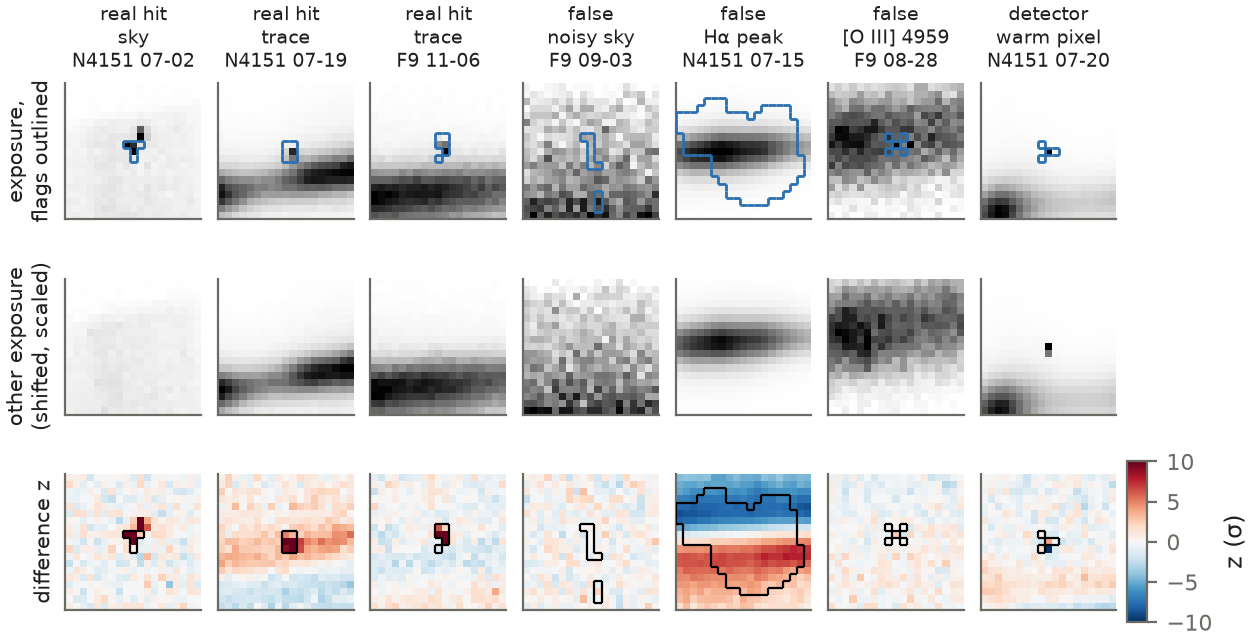
\includegraphics[width=\textwidth]{figures/fig_cr_gallery.png}
\caption{Flagged groups of final v3 classified by the same-visit test. Top: the exposure, flags outlined in red.
Middle: the other exposure of the visit, shifted and scaled onto the first. Bottom: the significance $z$ of the
difference ($-10$ blue to $+10$ red), flags outlined in black. Columns: real hits on the sky and on the trace (a compact
excess absent from the other exposure); false positives from the noisy sky model, on the H$\alpha$ peak (no localised
excess, only the dipole of a sub-pixel shift between the exposures) and on [O\,{\sc iii}]\,4959; and the warm pixel of
the OGG camera, present in both exposures.}
\label{fig:cr_gallery}
\end{figure}

\begin{table}[!htbp]
\centering
\caption{Same-visit test: flagged groups per frame (mean; median in brackets) by class and region, for the detector of
final v3 (\banzai{}~1.1.0) and the new one, on the same frames. ``Object'' is within two FWHM of the trace.}
\label{tab:cr_pairs}
\small
\begin{tabular}{@{}lrrrr@{}}
\toprule
 & \multicolumn{2}{c}{NGC\,4151, OGG (60 frames)} & \multicolumn{2}{c}{Fairall~9, COJ (46 frames)} \\
 & final v3 & new & final v3 & new \\
 & \multicolumn{4}{c}{(groups per frame)} \\
\midrule
real, object & 1.17 (1) & 1.42 (1) & 2.91 (3) & 3.07 (3) \\
false positive, object & 2.72 (1) & 6.30 (5) & 31.2 (6) & 14.8 (10) \\
ambiguous, object & 0.70 (0) & 1.60 (1) & 2.22 (0) & 2.22 (1) \\
missed, object & 11.8 (0) & 11.5 (0) & 1.70 (0) & 1.65 (0) \\
real, sky & 2.35 (2) & 2.35 (2) & 2.54 (2) & 2.65 (2) \\
false positive, sky & 8.87 (9) & 9.53 (9) & 13.2 (9) & 8.46 (8) \\
\bottomrule
\end{tabular}
\end{table}

Table~\ref{tab:cr_pairs} gives the result, and it is mixed:
\begin{itemize}
\item \textit{Real hits} are found as before, slightly more on the object (OGG 70 to 85, COJ 134 to 141 in all), and no
more are missed.
\item \textit{False positives on the object increase in normal frames}: the median per frame goes from 1 to 5 (OGG) and
from 6 to 10 (COJ). The COJ total halves (1435 to 680) only because the frames with the noisy sky model, which had
$\approx240$ each, are fixed. The new false positives are small (median 4 pixels), mostly within one FWHM of the trace
(OGG: 21 groups before, 151 after) and on the continuum, not on lines. Their cause is the other side of the change:
with the object subtracted, the fine-structure test of LA Cosmic is computed on the residual, which is small, and no
longer protects the core of a bright object, so the small pixel-scale structure left in the core of a spectrum with
S/N of a few hundred passes it.
\item \textit{False positives on the sky} are unchanged (OGG) or fewer (COJ, the noisy sky model). They are small groups
of a few faint pixels, cost a few pixels of the sky fit and do not affect the extraction.
\end{itemize}

\subsection{Effect on the extracted fluxes}
\label{sec:cr_flux}
What matters is whether the extra flags change the spectra. Table~\ref{tab:cr_flux} gives the agreement between the two
exposures of each visit, which the flags of either detector can only degrade. The new detector leaves it unchanged
within the noise for [O\,{\sc iii}] in the blue order, for H$\alpha$ and for the continuum, and lowers the bin-to-bin
scatter of the spectra slightly. The worst pairs are the same with both detectors and are grey (clouds, slit losses:
the same ratio in every quantity), except that the new detector removes the clipped H$\alpha$ pair (ratio 0.378). It
creates no new outlier.

The exception is [O\,{\sc iii}]\,5007 of NGC\,4151 in the \textit{red} order, where the line lies only 24\,\AA{} from
the blue end of the order and the dichroic cuts the light steeply: there both detectors clip the line in some frames,
the old one in 2 of 60 (17--22 pixels, flux 4--6 per cent low) and the new one in 6 (5--22 pixels, 4--5 per cent
low); everywhere else the two agree to 0.09 per cent. The bins lose less than half of their profile weight, so the
guard does not catch them. Lines within $\approx30$\,\AA{} of an order end should be measured in the other order, as
[O\,{\sc iii}] normally is in the blue.

\begin{table}[!htbp]
\centering
\caption{Agreement between the two exposures of a visit: robust scatter (per cent) of the ratio of their fluxes, and
the median bin-to-bin scatter of the spectra over their errors (\texttt{L1QXJ}).}
\label{tab:cr_flux}
\small
\begin{tabular}{@{}lrrrr@{}}
\toprule
 & \multicolumn{2}{c}{NGC\,4151 (30 visits)} & \multicolumn{2}{c}{Fairall~9 (23 visits)} \\
 & final v3 & new & final v3 & new \\
\midrule
\multicolumn{5}{@{}l}{\textit{Flux ratio of the two exposures, robust scatter (\%)}}\\
{[O\,{\sc iii}]\,5007}, blue order & 1.99 & 1.93 & 6.7 & 6.8 \\
{[O\,{\sc iii}]\,5007}, red order & 1.71 & 2.49 & 6.7 & 6.6 \\
H$\alpha$+[N\,{\sc ii}] & 2.53 & 2.29 & -- & -- \\
continuum 4200--4500\,\AA{} & 1.49 & 1.56 & 3.3 & 3.6 \\
continuum 7400--7550\,\AA{} & 1.48 & 1.55 & 3.0 & 2.8 \\
\multicolumn{5}{@{}l}{\textit{Bin-to-bin scatter over errors (no unit; 1 = correct)}}\\
scatter / errors (median) & 1.33 & 1.31 & 1.13 & 1.10 \\
\bottomrule
\end{tabular}
\end{table}

\subsection{Injection test}
\label{sec:cr_inject}
The same-visit test cannot see hits on bright line peaks, and it measures false positives better than completeness.
We therefore added 720 synthetic cosmic rays to copies of six raw frames (NGC\,4151 2025-07-15 and 2025-07-20,
BD$+28^\circ4211$ 2025-07-28 and 2025-08-19, Fairall~9 2026-09-06 and 2026-10-08; two random sets each), 20 per frame
in each of three places: the \textit{sky} (more than 3\,FWHM from the trace), the \textit{trace} (within 1\,FWHM, away
from the brightest pixels) and the \textit{peak} (the brightest 3 per cent of the trace core: the line peaks of the AGN
and the core of the star). The hits had peak charges from 50 to 20\,000\,e$^-$ (log-uniform) and the shapes of real
ones (one pixel, two pixels or a short track). Each copy, and the frame without hits, was reduced with both detectors;
a hit counts as detected if any of its pixels is flagged. Figure~\ref{fig:cr_validation} and
Table~\ref{tab:cr_inject} give the result:
\begin{itemize}
\item On the \textit{sky} both detectors find the same 90 per cent of the hits above 10$\sigma$ (the misses are the same
21 hits for both, 14 of them in the 2-pixel band at the order edges that is excluded from the search).
\item On the \textit{trace}, above 10$\sigma$, the old detector finds 89 per cent and the new one 100 per cent.
\item On the \textit{peaks} the old detector finds only 66 per cent of the hits above 10$\sigma$, and in the brightest
frames almost none: of the hits above 20$\sigma$, 0 of 8 on the core of BD$+28^\circ4211$ (2025 July 28) and 2 of 10 on
the H$\alpha$ peak of NGC\,4151 (2025 July 15). The new detector finds 97 per cent (83--100 per cent in every frame).
\item The masks cover the hits equally (95--97 per cent of the pixels of a detected hit), and when hits are added the
old detector also flags 49 pixels per frame that are not on a hit, the new one 13: with the low growth threshold
(step 6), a detection near a bright region spreads into it.
\end{itemize}
The reason is the same as for the false positives above, seen from the other side: the fine-structure test that
protected the object also hid the cosmic rays on it, because a hit on a bright core or line is a small sharp excess on
a large sharp signal. With the object subtracted, the hit stands out. A single hit on the [O\,{\sc iii}] peak of NGC\,4151
missed by the new detector in a first test (Section~\ref{sec:cr_model}) was one of the 3 per cent.

\begin{table}[!htbp]
\centering
\caption{Injection test: fraction of the injected cosmic rays detected (720 hits in six frames, each reduced with both
detectors).}
\label{tab:cr_inject}
\small
\begin{tabular}{@{}lrrrr@{}}
\toprule
 & \multicolumn{2}{c}{hits above 10$\sigma$} & \multicolumn{2}{c}{hits of 5--10$\sigma$} \\
place & final v3 & new & final v3 & new \\
 & \multicolumn{4}{c}{(fraction of the hits detected)} \\
\midrule
sky (240 hits) & 0.90 & 0.90 & 0.92 & 0.92 \\
trace (240) & 0.89 & 1.00 & 0.47 & 0.60 \\
line peak or star core (234) & 0.66 & 0.97 & 0.19 & 0.67 \\
\midrule
flags not on a hit (pixels per frame) & 49 & 13 & & \\
\bottomrule
\end{tabular}
\end{table}

\begin{figure}[!htbp]
\centering
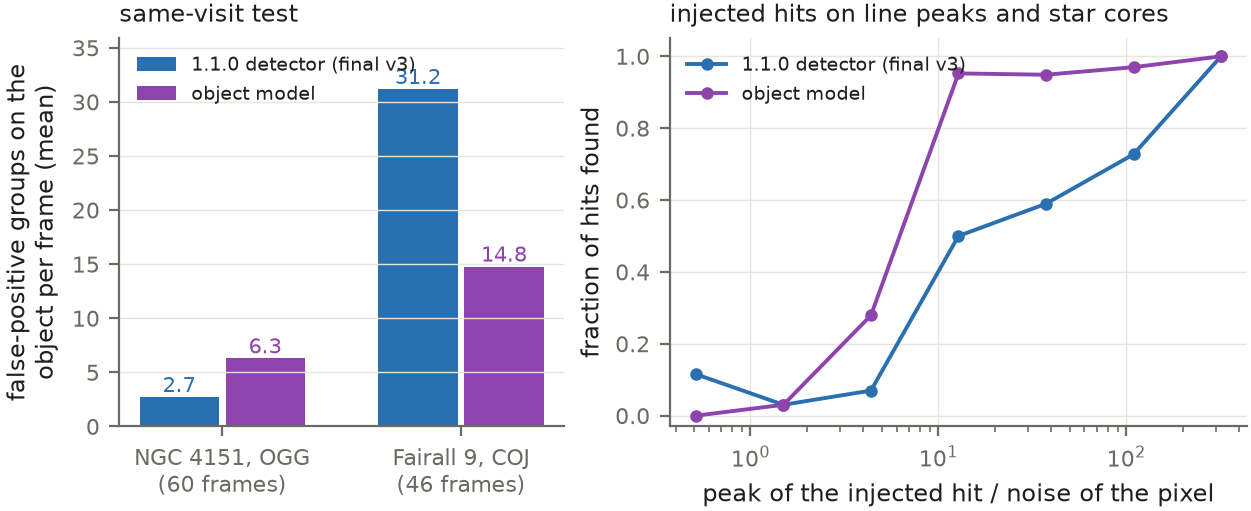
\includegraphics[width=\textwidth]{figures/fig_cr_validation.png}
\caption{Verification of the new detector against that of final v3 (\banzai{}~1.1.0). Left: same-visit test, flagged
groups per frame by class and region (Table~\ref{tab:cr_pairs}; the many ``missed'' groups of OGG are one visit with
11\,arcsec seeing, for both detectors). Middle: fraction of injected hits detected against their significance, on the
sky (dotted), the trace (dashed) and the line peaks or star core (solid), old (red) and new (blue). Right: the same
against the ratio of the hit to the signal under it, for hits above 10$\sigma$.}
\label{fig:cr_validation}
\end{figure}

\subsection{Conclusion}
\label{sec:cr_conclusion}
On the object, the new detector finds more of the real cosmic rays (on bright cores and line peaks 97 instead of 66 per
cent), stops flagging the cores of bright stars (46 to 0.1 per cent) and most of the clipped H$\alpha$ (179 to 15 pixels;
flux error 2.64 to 1.02), and removes the false detections caused by a noisy sky. In exchange it adds a few small false
detections per frame on the trace of bright objects (median 1 to 5 at OGG), which leave the extracted fluxes unchanged
within the noise, except for lines within $\approx30$\,\AA{} of an order end, where both detectors clip (2 and 6 frames of
60). On balance it is better on every measure that affects the spectra, but it is not perfect, and the results depend
on the parameters of LA Cosmic, which were left as in \banzai{}. A single frame cannot reliably separate a cosmic ray
from the peak of a bright line; the two or more exposures of every RM visit can, and comparing them is the robust
solution we recommend (Chapter~\ref{sec:recommendations}). We have not re-reduced the products with the new detector:
that, and whether to adopt it before a comparison of exposures exists, is a decision for the team.



\section{Quality keywords in every product}
\label{sec:qc}
Each science and standard product now carries per-frame quality keywords, whose names start with \texttt{L1Q}. They
are in the primary header of the \texttt{-1d} file and in the \texttt{SCI} header of the \texttt{-2d} file. A bitmask,
\texttt{L1QFLAG}, marks the problems found, and \texttt{L1QFLAGS} lists the names of the flags set
(Table~\ref{tab:qc_flags}). The last stage of the pipeline writes them. For products already on disk, the command
\texttt{banzai\_floyds\_qc} computes the same values from the files and writes them into the headers. It also writes a
table with one row per product, to be joined to a master table on the file name. The table holds all \texttt{L1} and
\texttt{L1Q} keywords and the observing conditions already in the headers of the raw frames: the guider seeing
(\texttt{AGFWHM}), the airmass (\texttt{AIRMASS}), the illuminated fraction of the Moon and its distance from the target
(\texttt{MOONFRAC}, \texttt{MOONDIST}) and the cloud measure of the weather station (\texttt{WMSCLOUD}). We added the
keywords to all 317 science and standard products of improved v3 at both sites. Their definitions and normal ranges are
in the file \texttt{docs/QC\_KEYWORDS.md} of the package. We set the thresholds of the flags just outside the normal
range of these reductions and checked them against the frames found by hand in this report.

The keywords are (a trailing 1/2 means one keyword for each order, red and blue):
\begin{itemize}
\item \texttt{L1QSN1/2}: the median S/N per wavelength bin.
\item \texttt{L1QXJ1/2}: the bin-to-bin scatter of the extracted flux over its errors. It is the robust rms of the
second difference of the flux divided by its expected error: 1 for pure noise, and insensitive to a smooth spectrum.
\texttt{L1QBJ1/2} is the same for the sky model under the object, still over the flux errors.
\item \texttt{L1QCR1/2}: the per cent of the trace core (pixels within one FWHM of the trace) flagged as cosmic rays.
\item \texttt{L1QCRLN}: cosmic-ray flags on the trace core of strong narrow emission lines. The lines are found in the
spectrum itself, as bins well above a running median, so no redshift is needed.
\item \texttt{L1QCRB1/2}: bins masked by the extraction guard (Section~\ref{sec:cr_guard}).
\item \texttt{L1QSEE1/2}: the seeing measured in the slit, the FWHM of the fitted spatial profile. (The guider's
\texttt{AGFWHM} is missing or zero in some frames.)
\item \texttt{L1QPOFF}: the offset of the object along the slit.
\item \texttt{L1QSTDGR}, standards only: the light collected relative to the clear ensemble of the other standards. It
finds standards taken through clouds and failed acquisitions.
\item \texttt{L1QSTDDT} and \texttt{L1QSTDSP}, science frames only: the days to the nearest and to the farthest standard
of the flux ensemble.
\end{itemize}

\begin{table}[!htbp]
\centering
\caption{Quality flags (\texttt{L1QFLAG} bits) and how many products of improved v3 have each. ``Science''
includes EG\,21 at COJ, which is not in the standards catalogue. A product can have several flags. ``Trace core'' is
the pixels within one FWHM of the trace; the refraction scale is a parameter of the physical trace model
(Chapter~\ref{sec:traces}); in the \texttt{BKMASK} row $\sigma$ is the width of the spatial profile.}
\label{tab:qc_flags}
\small
\begin{tabular}{@{}rlp{6.4cm}rrrr@{}}
\toprule
 & & & \multicolumn{2}{c}{COJ} & \multicolumn{2}{c}{OGG} \\
bit & flag & set when & sci. & std. & sci. & std. \\
 & & & \multicolumn{4}{c}{(number of products)} \\
\midrule
1 & \texttt{XJIT} & flux scatter $>2.5\times$ errors (either order) & 5 & 0 & 0 & 1 \\
2 & \texttt{BKJIT} & sky-model scatter $>1\times$ flux errors & 9 & 0 & 0 & 0 \\
4 & \texttt{CRCORE} & $>1$ per cent of the trace core flagged as cosmic rays & 0 & 0 & 0 & 12 \\
8 & \texttt{CRLINE} & $\geq3$ flags on the core of strong narrow lines & 5 & 0 & 3 & 0 \\
16 & \texttt{LOWSNR} & median S/N per bin $<10$ & 0 & 0 & 0 & 0 \\
32 & \texttt{TRACE} & trace not from the physical model, or $|$refraction scale$|>3$ & 0 & 0 & 0 & 1 \\
64 & \texttt{PROFILE} & profile width not fitted & 0 & 0 & 0 & 1 \\
128 & \texttt{BKMASK} & object mask narrowed below 6$\sigma$ (wide object, little sky) & 17 & 4 & 1 & 1 \\
256 & \texttt{STDGREY} & standard collected $<0.5$ of the clear ensemble & -- & 2 & -- & 4 \\
512 & \texttt{STDFAR} & nearest standard $>5$ days away & 44 & -- & 8 & -- \\
1024 & \texttt{FRINGE} & fringe residual ratio $>0.75$ & 0 & 0 & 0 & 1 \\
2048 & \texttt{NOOBJ} & no object detected & 0 & 0 & 0 & 0 \\
4096 & \texttt{SEEING} & seeing $>1.5\times$ the slit width & 9 & 21 & 0 & 10 \\
8192 & \texttt{CRBIN} & bins masked by the extraction guard & -- & -- & -- & -- \\
\midrule
 & \texttt{OK} & no flag & 58 & 18 & 48 & 75 \\
 & & products & 118 & 39 & 60 & 100 \\
\bottomrule
\end{tabular}
\end{table}

The flags find the problems of this chapter and of the earlier ones:
\begin{itemize}
\item \texttt{XJIT} and \texttt{BKJIT} find the Fairall~9 frames with the noisy sky model, and \texttt{XJIT} also the
BD$+28^\circ4211$ frame with half its core flagged.
\item \texttt{CRCORE} finds only BD$+28^\circ4211$, and \texttt{CRLINE} the clipped H$\alpha$.
\item \texttt{STDGREY} finds GD\,153 on 2025 May 25 (0.09 of the light of the clear standards; also flagged
\texttt{TRACE}, \texttt{PROFILE} and \texttt{FRINGE}), BD$+28^\circ4211$ on 2025 August 10 (0.06), and four standards
taken through clouds.
\item \texttt{STDFAR} shows that 44 COJ science frames are more than five days from a catalogue standard, because only
Feige\,110 is in the catalogue. EG\,21, taken almost every night, would close the gap
(Chapter~\ref{sec:recommendations}).
\item \texttt{CRBIN} is zero in all these products, because the extraction guard did not exist when they were reduced.
\end{itemize}

\begin{table}[!htbp]
\centering
\caption{Status of the changes of this chapter.}
\label{tab:cr_status}
\small
\begin{tabular}{@{}p{5.2cm}p{3.6cm}p{5.6cm}@{}}
\toprule
Change & In the code & In the products of this report \\
\midrule
Sky lines must stand out from the first-pass scatter & yes, tested & no: re-reduction pending \\
Object model for LA Cosmic & yes, tested & no: re-reduction pending \\
Extraction guard (mask bit 4) & yes, tested & no: re-reduction pending \\
Same-visit check after LA Cosmic & yes, tested (16 unit tests, 106 frames) & no: re-reduction pending \\
Gaia lookup tries a second VizieR mirror & yes, tested & no: re-reduction pending \\
Quality keywords & yes (last stage) & yes, added with \texttt{banzai\_floyds\_qc} \\
Warm pixel of the OGG camera in the bad-pixel mask & no & no \\
\bottomrule
\end{tabular}
\end{table}
